%----------------------------------------------------------------------------------------
%
% A LaTeX-template for 1DV510. Modified and translated by Björn Lindenberg at LNU.
% Based on an original master thesis template created by Marcus Wilhelmsson at LNU.
%
%----------------------------------------------------------------------------------------

% Settings and document configuration

\documentclass[a4paper,12pt]{article} 
\usepackage[T1]{fontenc} 
\usepackage{times} 
\usepackage[swedish,english]{babel} 
\usepackage[utf8]{inputenc} 
\usepackage{dtk-logos} 
\usepackage{wallpaper} 
\usepackage[absolute]{textpos} 
\usepackage[top=2cm, bottom=2.5cm, left=3cm, right=3cm]{geometry} 
\usepackage[parfill]{parskip} 
\usepackage{csquotes} 
\usepackage{float} 
\usepackage{lipsum} % Used for dummy text. Can be removed.
\usepackage{hyperref}
\hypersetup{
    colorlinks=true,
    linkcolor=black,
    filecolor=magenta,      
    urlcolor=blue,
    citecolor= black,
}
\usepackage[nottoc]{tocbibind}
% Fontsizes for section headings.
\usepackage{sectsty} 
\sectionfont{\fontsize{14}{15}\selectfont}
\subsectionfont{\fontsize{12}{15}\selectfont}
\subsubsectionfont{\fontsize{12}{15}\selectfont}

%----------------------------------------------------------------------------------------
%	This part is used for the text box on the title page
%----------------------------------------------------------------------------------------
\newsavebox{\mybox}
\newlength{\mydepth}
\newlength{\myheight}

\newenvironment{sidebar}%
{\begin{lrbox}{\mybox}\begin{minipage}{\textwidth}}%
{\end{minipage}\end{lrbox}%
 \settodepth{\mydepth}{\usebox{\mybox}}%
 \settoheight{\myheight}{\usebox{\mybox}}%
 \addtolength{\myheight}{\mydepth}%
 \noindent\makebox[0pt]{\hspace{-20pt}\rule[-\mydepth]{1pt}{\myheight}}%
 \usebox{\mybox}}

%----------------------------------------------------------------------------------------
%	Title
%----------------------------------------------------------------------------------------
\newcommand\BackgroundPic{
    \put(-2,-3){
    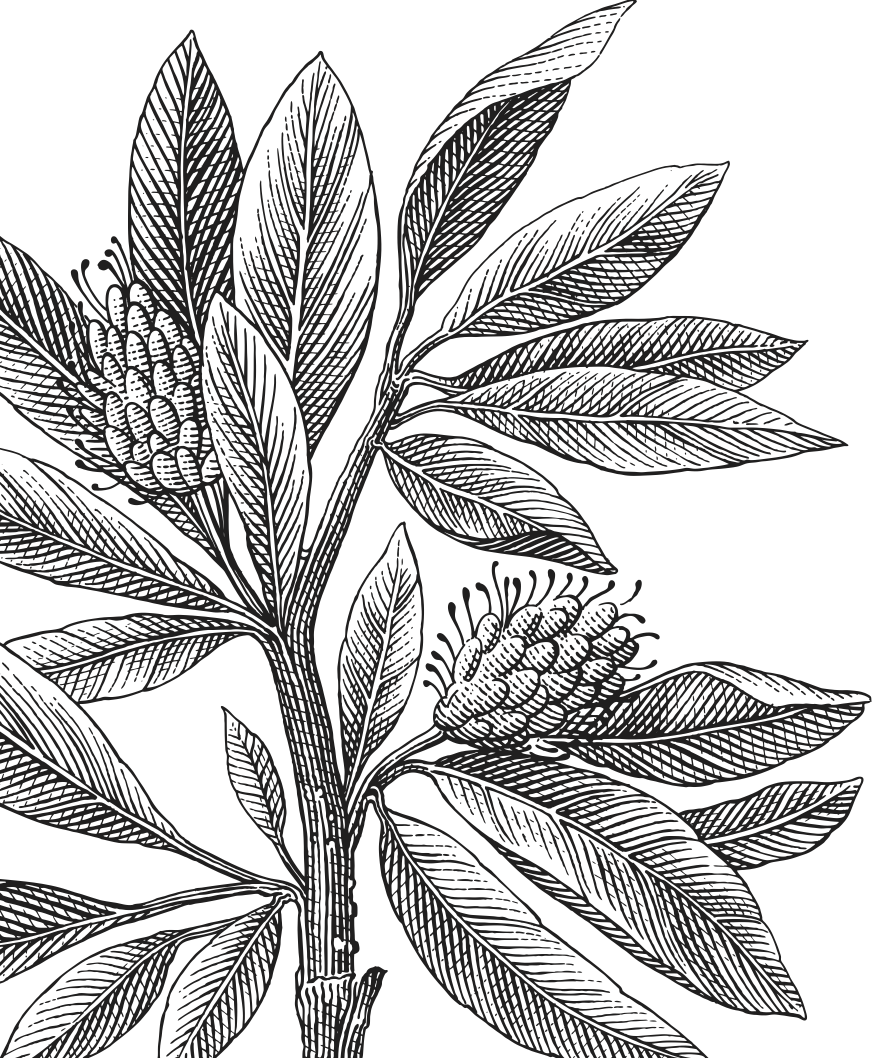
\includegraphics[keepaspectratio,scale=0.3]{img/lnu_etch.png} % Background image
    }
}
\newcommand\BackgroundPicLogo{
    \put(30,740){
    
\includegraphics[keepaspectratio,scale=0.10]{img/logo.png} % LNU logo
    }
}

\title{
\vspace{-8cm}
\begin{sidebar}
    \vspace{10cm}
    \normalfont \normalsize
    \huge Report\\ % Main title
    \vspace{-1.3cm}
\end{sidebar}
\vspace{3cm}
\begin{flushleft}
    \huge Act III: The Wealthy Individual \\% Subtitle
    \emph{Date: 31/05/2021}
\end{flushleft}
\null
\vfill
\begin{textblock}{6}(10,13)
\begin{flushright}
\begin{minipage}{\textwidth}
\begin{flushleft} \large
\emph{Author:}  Anas \textsc{Kwefati}\\  % Author
\emph{Email:} ak223wd@student.lnu.se\\ %Email
\emph{Semester:} Spring 2021\\ % Semester
\emph{Area:} Digital Forensics \\ % Area
\emph{Course code:} 2DV704 % Course
\end{flushleft}
\end{minipage}
\end{flushright}
\end{textblock}
}

\date{} % Empty date command. Use \today inside for today's date.
\author{} % Normally one would use this to define authors. However in this case the title command takes care of everything, so we leave the field empty to get rid of warnings. 

\begin{document}

\pagenumbering{gobble} % Turn off page numbering
\newgeometry{left=5cm}
\AddToShipoutPicture*{\BackgroundPic} % Adds the background image to the title page
\AddToShipoutPicture*{\BackgroundPicLogo} % Adds the logo to the title page
\maketitle % Prints the title
\restoregeometry
\clearpage

\pagenumbering{roman} % Roman page numbering for abstract page


\newpage

\pagenumbering{gobble} % Turn off page numbering
\tableofcontents 

\newpage
\pagenumbering{arabic} % Turn on page numbering

% Some example sections with dummy text
\section{Executive Summary}
\label{exe}

%This portion of the report will provide a synopsis of the purpose of the examination and the investigator’s major findings. In law enforcement, a separation of duties often occurs, particularly in larger computer forensics labs. This means that one officer works the investigation, and another officer performs the forensic analysis.
%
%Therefore, the work of more than one law enforcement agent is included in the report, and that must be clearly outlined in the report.

The main purpose of this investigation is to decrypt the access codes to the victim's Swiss bank account, so he will not have to pay the ransom, and will still be able to do business. Moreover, the victim, would like to have an idea as who is responsible for this incident. After investigation, it has been concluded that the system was indeed compromised, and the encrypted codes were successfully solved, however, the incident timeline to the day of encryption is still unclear, despite having the butler account being suspicious. 

\section{Purpose of the Investigation}

%This section is optional because the report writer may have explained the reason for conducting the investigation in the Executive Summary. To set the tone for the report, the report writer might want to explain the reason for the investigation and the scope of the warrant, which will later help explain the types of computing devices that were examined and the areas of memory that were analyzed. For example, picture and video files will be important in a suspected pedophile case, whereas emails might be particularly important in a corporate insider investigation, and bank information is important in an embezzlement investigation.

The reason for conducting the investigation can be read in Section \ref{exe}. But to sum it up, someone has contacted us because his employer's computer had been compromised by an intruder. This person managed to delete the files and encrypted the employer's Swiss bank account access codes. Therefore, to be able to decrypt the Swiss bank access keys, we have decided to use some tools to recover deleted files, look into the memory swap, but also look at each user's profile. Despite not being the priority for our client, he would like to know who is responsible, thus we will be also looking into the logs section and see if there is anything useful. We are investigating the image using Kali Linux 2020.3 in a Virtual Machine environment.  

\section{Methodology}

%The methodology can be included as a separate section in the report or can be included later. The methodology explains the science behind the examination. It should explain the approach the forensics examiner took, which might include the choice of software or hardware tools. The investigator may also reference standard practices for computer forensics examinations that were used in the examination—these could be lab specific, could come from the Department of Justice, or could be recommendations from NIST.

We have followed the standard procedures, and protocol for this investigation. Thus, in this forensic examination, we have decided to download \textbf{act3.img}, in our local environment using the command tool rsync. Then we mounted that image into our Kali Linux VM using VirtualBox. Kali Linux was chosen as it regroups many tools that can be used for digital forensics. We made sure to keep a copy of the image, and have it as a read only, and we also created a hash value of that image in order to make sure everything is the same (Figure \ref{hash}). The client's priority was to decrypt the keys, therefore, when accessing the image, we directly started to recover any deleted files, and checked the users in order to find any keys to decrypt the access codes. When they were found, we managed to decrypt the keys, and we decided to look at who is responsible of this event. Thus, the logs were checked, but also users' bash history.  

In order to complete the investigation, the following tools were used: 

\begin{itemize}
\item \textbf{Tsk\_recover:} Tool to recover deleted files on the system.
\item \textbf{Hexedit:} Displays and examine binary files in hexadecimal. 
\item \textbf{Cat:} View the content of a file.
\item \textbf{Less:} Displays the content of a file.
\item \textbf{Grep:} Used to search texts and strings in a gile.
\item \textbf{John The Ripper:} Used to crack users passwords.
\item \textbf{Gpg:} GnuPrivacy Guard was used to decrypt the swisskey files with .gpg extension.
\end{itemize}
 
\section{Electronic Media Analyzed}
The file \textbf{act3.img} has been examined. An .img extension means that the file is storing raw disk images of either a floppy disks, hard drives, and optical discs. Therefore, there should be no data beyond what the content of the disk. The investigator has obtained the file on May 31, 2021 10:10 in the morning. The total size of the file is 2Gb. 
 
\section{Report Findings}

%As previously noted, the report should be clear about the findings related to the nature of the investigation and within the scope of all search warrants. All technical terms should be comprehensively explained. It is important for the investigator to state the facts and be careful about interpretations—that is for the attorneys and, potentially, the jury to decide. Consider an example of proper phrasing versus improper statements:

An analysis was conducted on the given image file of the hard disk. This hard disk is owned by a person with a lot of money, and was imaged by the investigator in order to analyze it. The Figure \ref{table}, contains the timeline of the incident in Pacific Daylight Time (PDT) according to the system. 

We received this hard disk on May 31, 2021 at 10:10 AM, and an image was created from it, named as \textbf{act3.img}. After this, we decided to create a copy of it and generate a cryptographic hash of the copy and the original file. Doing that allows us to ensure that the two images are bit-for-bit the same, and represent exactly what is on the file. This result can be seen in Figure \ref{hash}. We also made sure that it is in read only, so we don't modify anything. 

Now, we know for certain that the copy image has not been changed, therefore, all future work will be done on the copy image file. 
The first thing we did was to check if the hard disk was infected with a malware. Doing this step is important, in order to make sure that no malware were installed on the system. Therefore, we used the anti-virus \textbf{ClamAV}. We scanned the file, and no malware were detected.

The second step we have done, was to focus on the main investigation, which is to decrypt the Swiss keys by finding the passwords. Therefore, we started by recovering all the files from the device, which will be analyzed. Meanwhile, we decide to check each users profile, and gather some information. When looking at \textbf{Rich} account, we can learn there are a total of 8 keys encrypted (Figure \ref{allswiss}), so from here we are sure at the total number of keys to recover. Furthermore, when looking at Rich's path, we managed to find two folders (\textbf{.mozilla} and \textbf{.extrtmtc}), that contain the passwords 4 and 5 (Figure \ref{key4}, and \ref{key5}). When using those passwords, we were able to decrypt the swisskey 4 and 5. Afterward, we decided to look the other users, but nothing important was found in regards to the key decryption. Thus, we preferred to look other places in the system, in Figure \ref{key1}, we managed to find the password to decrypt swisskey 1, which is located in \textbf{tmp} (temporary) folder, which is inside another folder named as \textbf{extormatic-2341}. At that moment, we tried to search other keys in other paths, but nothing successful was obtained, so we decided to examine the recovered files. 

We managed to recover many files, but most of them did not seem to contain useful data, except 4 files. In Figure \ref{key678}, we can see 3 files that contain the passwords which can be used to decrypt their corresponding Swiss key 6, 7 and 8. Additionally, we found a special file which seems to be a deleted bash history by the intruder (Figure \ref{recovered}), indeed from that point it is visible that someone created the \textit{.mozilla} and \textit{.extrtmtc} folders, but also it is visible that someone was encrypting the swisskeys using gpg. This person seemed to know what he was doing. Either way, after find this, we decided to look to other files, but nothing too important was gathered, so we had to check the swap space (Figure \ref{swap} shows the swap location). We have used hexedit, in order to read the data, when searching for the keyword \textbf{Key}, we managed to find the passwords for the swisskey 2 and 3 (Figure \ref{key2}, and \ref{key3}). 

At that point, we found all the passwords that were used to decrypt all the swisskeys, and thus the client does not need to pay the ransom for the decryption keys. Figure \ref{decrypted} shows the final result. 


Now that the main issue was solved as we decrypted all the codes, the next step we have taken was to understand what has happened. 

The first step was to check the passwd file (\textbf{etc/passwd}), to see if there was something out of the normal, but we only found 5 users, which are \textbf{Rich}, \textbf{Jeeves}, \textbf{Gardener}, \textbf{Chef}, and \textbf{Ubuntu} (Figure \ref{pass}). 

Then, the next step was to analyze the logs, in the folder \textbf{/var/log}. The \textbf{Auth.log} had interesting information as we could see which session has been opened, and the accepted password (Figure \ref{auth2}, and \ref{sessionAuth}). The other logs did not seem to have much information, so we looked at the bash history for each user, in case there's something. 

\begin{itemize}
\item \textbf{Chef:} Nothing important was found, beside he created a folder called \textit{recipes}, and looked like he was writing some bread recipe (Figure \ref{chef}).
\item \textbf{Gardener:} As seen in Figure \ref{gardener}, this person was trying to read his bash history using the command \textbf{cat}, but also he tested \textbf{gpg} command. However, there is not enough evidence to suspect this person. 
\item \textbf{Jeeves:} In Figure \ref{jeeves}, we can see that someone, or Jeeves himself, was monitoring the activity of all the users in the system except for himself (\textit{watch "w | grep -v jeeves"}). Furthermore, he used the command \textit{su} to switch to Rich's account, but as well as to the root account, Figure \ref{jeevesLog}, shows it clearly as well. 
\item \textbf{Rich:} No bash history was found, hence we can suspect that the intruder used Rich account to encrypt the Swiss keys and deleted the bash history, so no one can find it. That being said, the bash history was recovered Figure \ref{recovered}.
\item \textbf{Ubuntu:} Nothing important was found for this user (Figure \ref{ubuntu}).
\end{itemize}

 


%\section{Investigation Details Connected to the Case}
%This is not necessarily a separate section, but it is important to note supporting evidence to the investigation that is not digital. These might include statements from the suspect and witnesses.


\section{Conclusion}

To conclude, we have managed to recover all the Swiss access codes, as we managed to find all the passwords to decrypt them, thus there is no need to pay the ransom anymore. Furthermore, according to all the gathered data, we believe that someone accessed to Jeeves and Rich's account in order to encrypt the Swiss bank access codes, we also suspect that it is an insider job, as this person seemed to know where to find the information, but also knew all the passwords, as he managed to access to all the accounts. We could also assume that the intruder is the butler himself, as he might know the passwords, where the files are located and so on. He might have encrypted the Swiss account access on purpose for money. Nevertheless nothing is sure, and the client should take the appropriate actions to find the responsible. The Figure \ref{table}, shows the timeline of the incident. 

Finally, before returning the system to production, there is a need on defining properly the privileges for each user and restricting to only what they need. Also, any sensitive data should have been encrypted and stored securely somewhere, as only the owner of those keys should have had access to them. We would also recommend to format the whole disk, as it has been compromised. Then, we managed to crack all the users' password, Figure \ref{crack} shows they were not secure enough, thus, there is a need to create more complex passwords, with at least 13 characters. They would include uppercase, and lowercase letters, but also special characters, numbers etc. Doing that would make it harder for anyone to crack them and have access into the accounts. 
%Many commands should have been limited to only the administrator, so there is a need to put more restriction in there as well. 

After the investigation was finished, we have generated the hash of the image and we obtained: 

SHA256(act3.img) = 79c060f1439c4f82a276ec728bbd2059bd486319b2fce80e2cfaa1d11b1936f9

This matches what we obtained at the beginning of the investigation. The inspection was finished on June 1, 2021 at 10:10 AM.

\section{Exhibits/Appendices}

%Exhibits can include photos of seized objects, screenshots of the computer screen, tagged photographs, printed emails, and any other files of interest. Appendixes can include forms, like the evidence list and the search warrant.


\begin{figure}[H]
	\begin{center}
		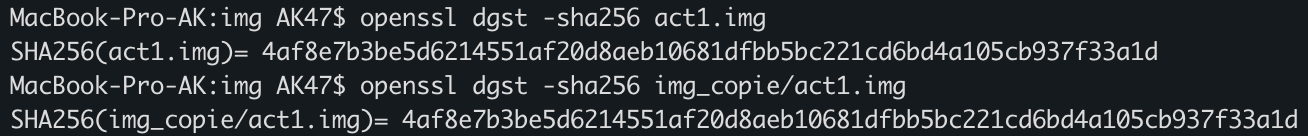
\includegraphics[scale = 0.60]{img/act1/hash.png} 
	\end{center}
	\caption{Cryptographic hash value of act3.img}
	\label{hash}
\end{figure}

\begin{figure}[H]
	\begin{center}
		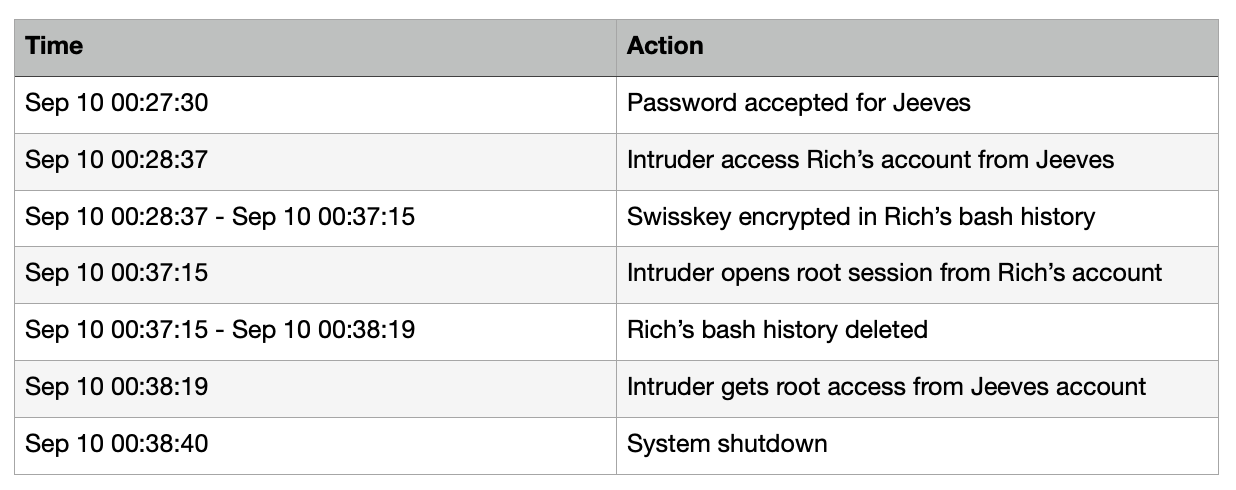
\includegraphics[scale = 0.65]{img/act1/table.png} 
	\end{center}
	\caption{Incident timeline}
	\label{table}
\end{figure}

\begin{figure}[H]
	\begin{center}
		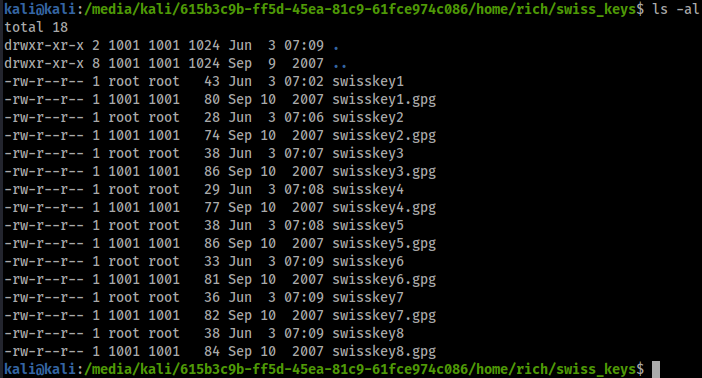
\includegraphics[scale = 0.60]{img/act1/allswiss.png} 
	\end{center}
	\caption{Swisskeys encrypted}
	\label{allswiss}
\end{figure}

\begin{figure}[H]
	\begin{center}
		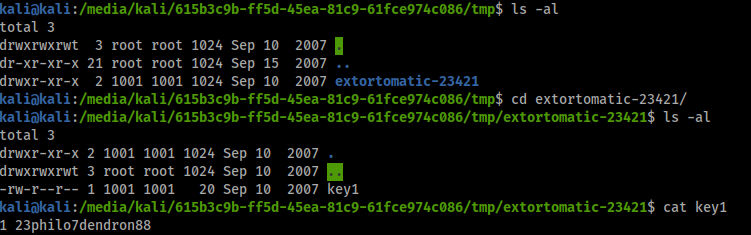
\includegraphics[scale = 0.50]{img/act1/key1.png} 
	\end{center}
	\caption{Swiss Bank Key 1}
	\label{key1}
\end{figure}

\begin{figure}[H]
	\begin{center}
		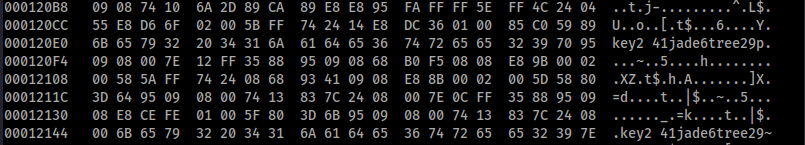
\includegraphics[scale = 0.50]{img/act1/key22.png} 
	\end{center}
	\caption{Swiss Bank Key 2}
	\label{key2}
\end{figure}

\begin{figure}[H]
	\begin{center}
		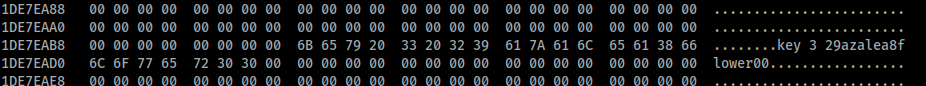
\includegraphics[scale = 0.50]{img/act1/key3.png} 
	\end{center}
	\caption{Swiss Bank Key 3}
	\label{key3}
\end{figure}

\begin{figure}[H]
	\begin{center}
		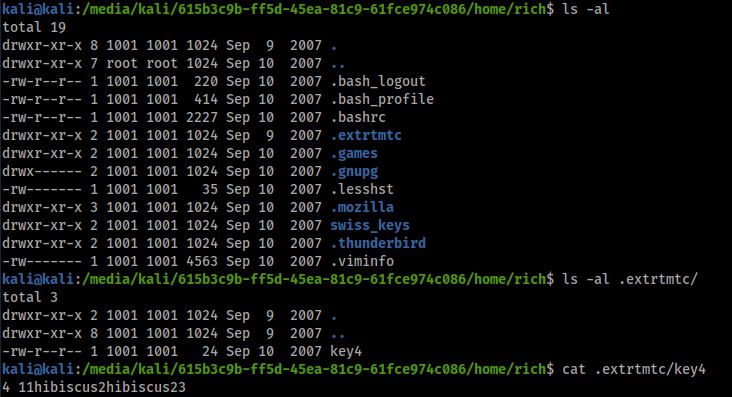
\includegraphics[scale = 0.50]{img/act1/key4.png} 
	\end{center}
	\caption{Swiss Bank Key 4}
	\label{key4}
\end{figure}

\begin{figure}[H]
	\begin{center}
		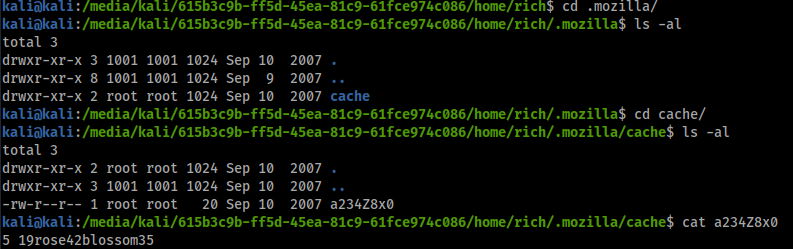
\includegraphics[scale = 0.50]{img/act1/key5.png} 
	\end{center}
	\caption{Swiss Bank Key 5}
	\label{key5}
\end{figure}

\begin{figure}[H]
	\begin{center}
		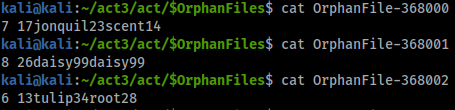
\includegraphics[scale = 0.65]{img/act1/key678.png} 
	\end{center}
	\caption{Swiss Bank Key 6,7, and 8}
	\label{key678}
\end{figure}

\begin{figure}[H]
	\begin{center}
		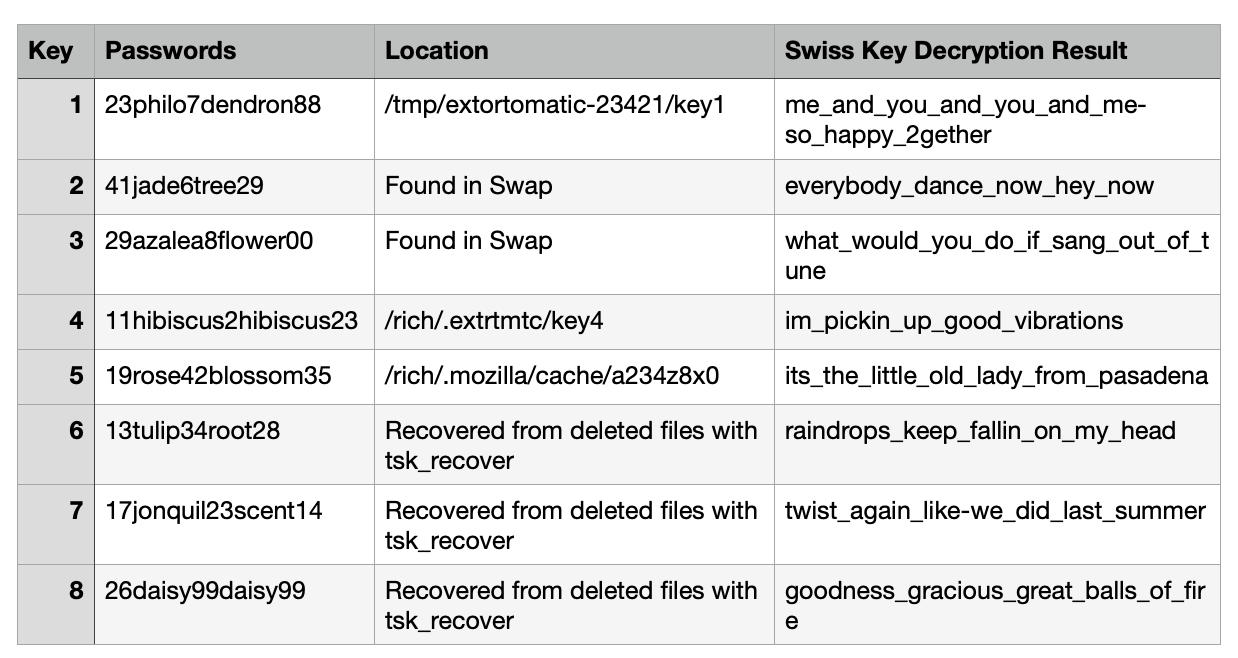
\includegraphics[scale = 0.75]{img/act1/result.png} 
	\end{center}
	\caption{Swiss Keys decrypted result}
	\label{decrypted}
\end{figure}

\begin{figure}[H]
	\begin{center}
		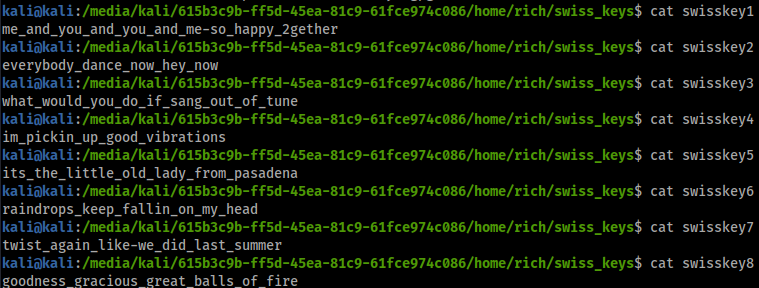
\includegraphics[scale = 0.60]{img/act1/swisskeyDecrypted.png} 
	\end{center}
	\caption{Swiss Keys decrypted}
	\label{decrypted}
\end{figure}

\begin{figure}[H]
	\begin{center}
		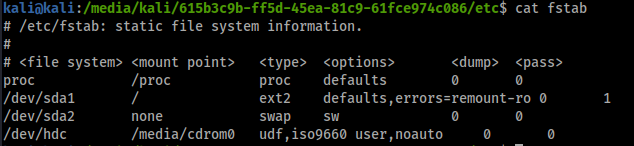
\includegraphics[scale = 0.57]{img/act1/swaplocation.png} 
	\end{center}
	\caption{Swap file location}
	\label{swap}
\end{figure}
%------------------------------------

\begin{figure}[H]
	\begin{center}
		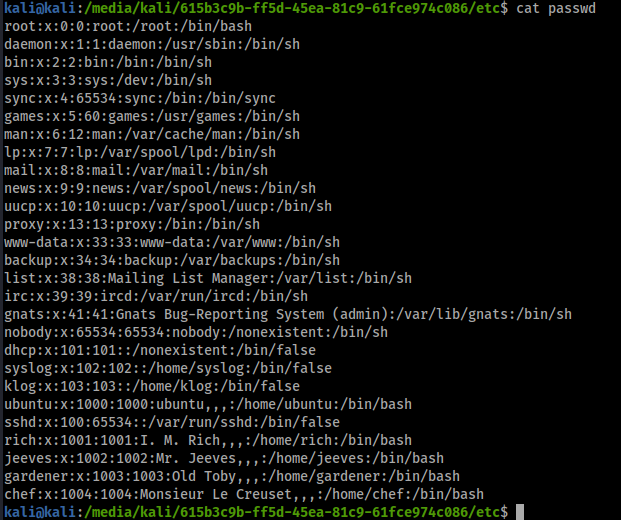
\includegraphics[scale = 0.49]{img/act1/pass.png} 
	\end{center}
	\caption{Passwd file}
	\label{pass}
\end{figure}

\begin{figure}[H]
	\begin{center}
		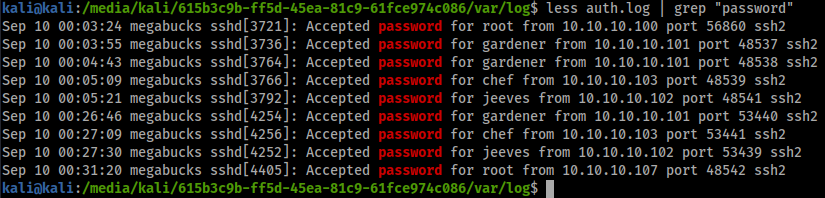
\includegraphics[scale = 0.53]{img/act1/authlogPasswd.png} 
	\end{center}
	\caption{Auth.log file content filtered with GREP with keywords Password}
	\label{auth2}
\end{figure}


\begin{figure}[H]
	\begin{center}
		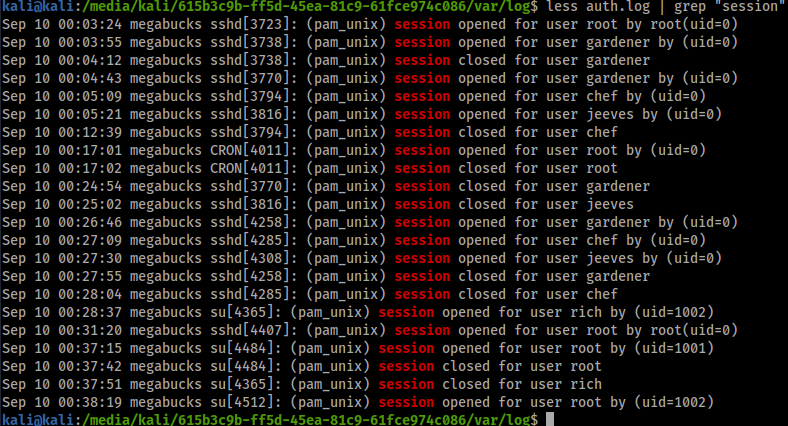
\includegraphics[scale = 0.50]{img/act1/authlogSession.png} 
	\end{center}
	\caption{Auth.log file content filtered with GREP with Session keyword}
	\label{sessionAuth}
\end{figure}


\begin{figure}[H]
	\begin{center}
		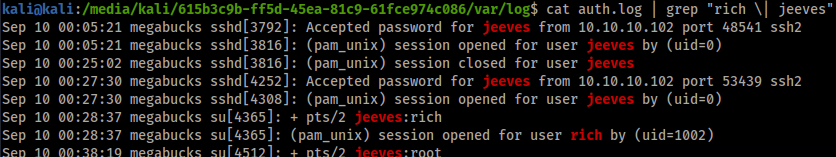
\includegraphics[scale = 0.50]{img/act1/jeeveRichLog.png} 
	\end{center}
	\caption{Auth.log file content filtered with GREP for Jeeves and Rich}
	\label{jeevesLog}
\end{figure}

\begin{figure}[H]
	\begin{center}
		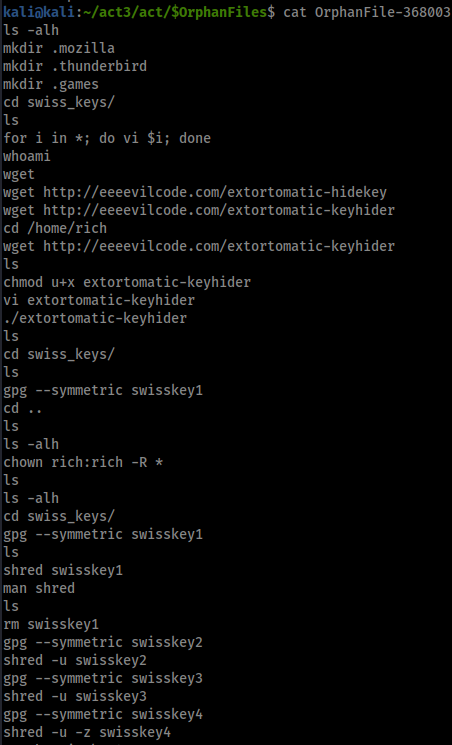
\includegraphics[scale = 0.50]{img/act1/bashRecovered.png} 
	\end{center}
	\caption{Recovered bash history}
	\label{recovered}
\end{figure}

%------------------------------------
\begin{figure}[H]
	\begin{center}
		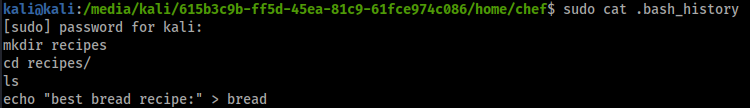
\includegraphics[scale = 0.55]{img/act1/chefBash.png} 
	\end{center}
	\caption{Chef's Bash History}
	\label{chef}
\end{figure}

\begin{figure}[H]
	\begin{center}
		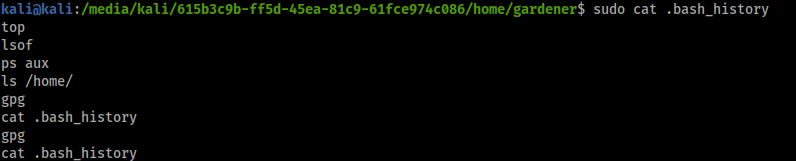
\includegraphics[scale = 0.55]{img/act1/gardenerBash.png} 
	\end{center}
	\caption{Gardener's Bash History}
	\label{gardener}
\end{figure}

\begin{figure}[H]
	\begin{center}
		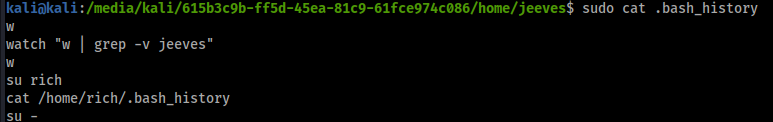
\includegraphics[scale = 0.55]{img/act1/jeevesBash.png} 
	\end{center}
	\caption{Jeeves' Bash History}
	\label{jeeves}
\end{figure}

\begin{figure}[H]
	\begin{center}
		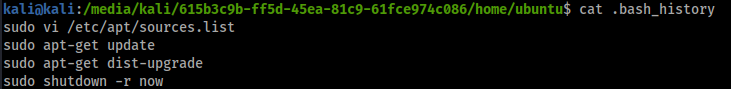
\includegraphics[scale = 0.55]{img/act1/ubuntuBash} 
	\end{center}
	\caption{Ubuntu's Bash History}
	\label{ubuntu}
\end{figure}

\begin{figure}[H]
	\begin{center}
		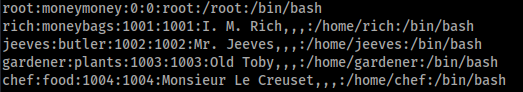
\includegraphics[scale = 0.55]{img/act1/crack.png} 
	\end{center}
	\caption{Cracked Password}
	\label{crack}
\end{figure}


%----------------------------------

%\begin{figure}[H]
%	\begin{center}
%		\includegraphics[width=350]{Latex_Template/img/er.png} 
%	\end{center}
%	\caption{e2undel command}
%	\label{fig:e2undel}
%\end{figure}

% Prints your bibliography database xxx.bib
%\bibliographystyle{IEEEtran}
%\bibliography{ref.bib}

\end{document}
